\section{正规方程法}
\label{sec:ls-normal-equations-method}

上一章处理的都是方阵的精确解。现在转向超定的最小二乘问题，矩阵不再是方阵，消元也不再直接适用。最直接的办法是先把问题化为一个方阵问题：最小二乘解满足正规方程，而满列秩时正规方程的系数矩阵对称正定，正好可以交给Cholesky分解。

\subsection{主要思想}

输入满列秩的$\bm A\in\mathbb R^{m\times d}$（$m\geq d$）和$\bm b\in\mathbb R^m$，求唯一的最小二乘解$\hat{\bm x}$。核心思想是把它化为一个$d$阶方程
\begin{equation}
 \bm G\hat{\bm x}=\bm c,\qquad \bm G=\bm A^\top\bm A,\quad \bm c=\bm A^\top\bm b,
 \label{eq:ls-normal-system}
\end{equation}
再用Cholesky分解求解。下面先说明这个方程从哪里来，再说明$\bm G$与$\bm c$怎样计算。

\paragraph{正规方程}
记$\bm A$的各列为$\bm a_1,\ldots,\bm a_d$，残差为$\bm r=\bm b-\bm A\bm x$。第~\ref{sec:ls-ordinary-ls}节已经证明，最优拟合值是$\bm b$在列空间上的正交投影，所以最优残差与每一列正交：
\[
 \bm a_j^\top(\bm b-\bm A\hat{\bm x})=0,\qquad j=1,\ldots,d .
\]
把这$d$个标量等式自上而下排成一个向量，左边的$\bm a_1^\top,\ldots,\bm a_d^\top$恰好是$\bm A^\top$的各行，于是得
\[
 \bm A^\top\bm b-\bm A^\top\bm A\hat{\bm x}=\bm0 ,
\]
移项即式~\eqref{eq:ls-normal-system}，也就是式~\eqref{eq:linear-algebra-normal-equations}的正规方程。这一推导只用正交投影，不需要多元求导。逐个分量看，$\bm G$的$(j,k)$元与$\bm c$的第$j$个分量分别是
\[
 g_{j,k}=\bm a_j^\top\bm a_k,\qquad c_j=\bm a_j^\top\bm b .
\]

满列秩时$\bm G$对称正定，理由见本节的算法分析。于是可以按第~\ref{sec:ls-cholesky}节分解$\bm G=\bm L\bm L^\top$，再像求解正定方程那样，先按式~\eqref{eq:ls-forward-substitution}前代求解$\bm L\bm y=\bm c$，再按式~\eqref{eq:ls-back-substitution}回代求解$\bm L^\top\hat{\bm x}=\bm y$。

\paragraph{按行累计}
$\bm G$与$\bm c$不必按列作内积。把$\bm A$的第$i$行记为$\bm A_{i,:}$，则$\bm G$的$(j,k)$元
\[
 \bm a_j^\top\bm a_k=\sum_{i=1}^m a_{i,j}a_{i,k}
\]
恰是各行外积$\bm A_{i,:}^\top\bm A_{i,:}$的$(j,k)$元之和；$\bm c$的第$j$个分量$\sum_{i}a_{i,j}b_i$同样是各行贡献之和。所以
\begin{equation}
 \bm G=\sum_{i=1}^m\bm A_{i,:}^\top\bm A_{i,:},\qquad
 \bm c=\sum_{i=1}^mb_i\bm A_{i,:}^\top .
 \label{eq:ls-gram-row-accumulation}
\end{equation}
每条观测只贡献一个$d$阶外积和一个$d$维向量，所以可以每读入一行就把它的贡献累加进去，不必同时保存全部观测行。这是正规方程法在数据量很大时的主要优点；代价在数值精度上，$\bm G$的条件数是$\bm A$的平方，见本节的算法分析。

\subsection{算法实现}

输入是满列秩的$\bm A$与$\bm b$，输出是$\hat{\bm x}$，没有需要预先选定的规则。算法由三个模块组成，下面依次给出：形成Gram矩阵与右端，由式~\eqref{eq:ls-gram-row-accumulation}算出$\bm G$与$\bm c$；$\bm L\bm L^\top$分解算出$\bm L$；前代与回代求出$\hat{\bm x}$。

下面用示例~\ref{ex:ls-line-least-squares}的直线拟合数据逐步演示：
\[
 \bm A=\begin{bmatrix}1&0\\1&1\\1&2\end{bmatrix},\qquad
 \bm b=\begin{bmatrix}1\\2\\2\end{bmatrix}.
\]
本章后面的QR求解及其三种因子计算也沿用这组数据。

\subsubsection{形成Gram矩阵与右端}
输入$\bm A$与$\bm b$，输出$\bm G$与$\bm c$。
\begin{enumerate}
 \item \textbf{初始化。}令$\bm G=\bm0$，$\bm c=\bm0$，$i=1$。

 \item \textbf{累加第$i$行。}根据式~\eqref{eq:ls-gram-row-accumulation}，令
 \[
  \bm G\leftarrow\bm G+\bm A_{i,:}^\top\bm A_{i,:},\qquad
  \bm c\leftarrow\bm c+b_i\bm A_{i,:}^\top .
 \]
 $\bm G$对称，只需累加下三角部分。
 
 例中三行依次为$(1,0)$、$(1,1)$、$(1,2)$，右端依次为$1,2,2$。逐行写出$\bm G$与$\bm c$的增量：
 \[
  \begin{aligned}
  &i=1:&&\begin{bmatrix}1&0\\0&0\end{bmatrix},\quad\begin{bmatrix}1\\0\end{bmatrix};\\
  &i=2:&&\begin{bmatrix}1&1\\1&1\end{bmatrix},\quad\begin{bmatrix}2\\2\end{bmatrix};\\
  &i=3:&&\begin{bmatrix}1&2\\2&4\end{bmatrix},\quad\begin{bmatrix}2\\4\end{bmatrix}.
  \end{aligned}
 \]

 \item \textbf{判断是否结束。}若$i<m$，令$i\leftarrow i+1$，回到第2步；否则结束。
 
 例中三行累加完毕，得
 \[
  \bm G=\begin{bmatrix}3&3\\3&5\end{bmatrix},\qquad
  \bm c=\begin{bmatrix}5\\6\end{bmatrix}.
 \]
\end{enumerate}

\subsubsection{\texorpdfstring{$\bm L\bm L^\top$}{LLT}分解}
输入$\bm G$，输出$\bm L$。对$j=1,\ldots,d$逐列按式~\eqref{eq:ls-cholesky-columns}计算：先算开方量，检查$\delta_j>0$后取对角元，
\[
 \delta_j=g_{j,j}-\sum_{k<j}l_{j,k}^2,\qquad l_{j,j}=\sqrt{\delta_j},
\]
再对$i=j+1,\ldots,d$算出$l_{i,j}$；处理完第$d$列后结束。

例中按列计算：
\[
 \begin{aligned}
 &\text{第一列：}&& l_{1,1}=\sqrt3,\quad l_{2,1}=\tfrac{3}{\sqrt3}=\sqrt3;\\
 &\text{第二列：}&& l_{2,2}=\sqrt{5-(\sqrt3)^2}=\sqrt2 .
 \end{aligned}
\]
于是
\[
 \bm L=\begin{bmatrix}\sqrt3&0\\\sqrt3&\sqrt2\end{bmatrix}.
\]

满列秩保证了每个$\delta_j>0$。若某个$\delta_j\leq0$，说明$\bm A$秩亏或条件很差，停止并改用第~\ref{sec:ls-qr-method}节的QR求解或第~\ref{sec:ls-svd-solve}节的SVD求解。

\subsubsection{前代与回代}
输入$\bm L$与$\bm c$，输出$\hat{\bm x}$。
\begin{enumerate}
 \item \textbf{前代。}根据式~\eqref{eq:ls-forward-substitution}，对$i=1,\ldots,d$依次计算
 \[
  y_i=\frac{c_i-\sum_{k<i}l_{i,k}y_k}{l_{i,i}} ,
 \]
 求出$y_d$后结束。
 
 例中
 \[
  y_1=\frac{5}{\sqrt3},\qquad
  y_2=\frac{6-\sqrt3\cdot\frac5{\sqrt3}}{\sqrt2}=\frac1{\sqrt2}.
 \]

 \item \textbf{回代。}根据式~\eqref{eq:ls-back-substitution}，$\bm L^\top$的$(i,k)$元取$l_{k,i}$，对$i=d,\ldots,1$依次计算
 \[
  \hat x_i=\frac{y_i-\sum_{k>i}l_{k,i}\hat x_k}{l_{i,i}} ,
 \]
 求出$\hat x_1$后结束。
 
 例中
 \[
  \hat x_2=\frac{1/\sqrt2}{\sqrt2}=\frac12,\qquad
  \hat x_1=\frac{\frac5{\sqrt3}-\sqrt3\cdot\frac12}{\sqrt3}=\frac53-\frac12=\frac76 .
 \]

 \item \textbf{输出并核验。}输出$\hat{\bm x}$，并用原始数据计算残差$\bm r=\bm b-\bm A\hat{\bm x}$，检查$\bm A^\top\bm r=\bm0$。
 
 例中解与残差为
 \[
  \hat{\bm x}=\begin{bmatrix}7/6\\1/2\end{bmatrix},\qquad
  \bm r=\begin{bmatrix}-1/6\\1/3\\-1/6\end{bmatrix}.
 \]
 残差与两列都正交，
 \[
  \bm A^\top\bm r=\bm0,\qquad \lVert\bm r\rVert_2^2=\tfrac16 .
 \]
\end{enumerate}

例中的残差不为零，是因为三个点本来就不共线，方程不相容；最小二乘完成的标志是$\bm A^\top\bm r=\bm0$，而不是$\bm r=\bm0$。若累计后的Cholesky分解失败，或结果对舍入很敏感，也不能只凭正规方程这个小系统的残差小就宣布结果可靠。

\subsection{算法分析}

\paragraph{满列秩保证正定}
$\bm G=\bm A^\top\bm A$显然对称。若$\bm A$满列秩，则对任意$\bm z\neq\bm0$有$\bm A\bm z\neq\bm0$，于是
\[
 \bm z^\top\bm G\bm z=\lVert\bm A\bm z\rVert_2^2>0 ,
\]
$\bm G$对称正定。由定理~\ref{thm:ls-cholesky-existence}，$\bm L\bm L^\top$分解中的开方量都为正。秩亏时这一论证失效：存在$\bm z\neq\bm0$使$\bm A\bm z=\bm0$，$\bm G$只是半正定的。

\paragraph{正确性}
两次三角求解给出$\bm L\bm L^\top\hat{\bm x}=\bm c$，即$\bm A^\top\bm A\hat{\bm x}=\bm A^\top\bm b$，所以$\hat{\bm x}$满足正规方程，由定理~\ref{thm:ls-least-squares-solutions}是唯一的最小二乘解。

\paragraph{数值敏感度}
这条路线的代价在精度。对满列秩矩阵定义$\kappa_2(\bm A)=\sigma_{\max}(\bm A)/\sigma_{\min}(\bm A)$，方阵时它与第~\ref{sec:ls-matrix-condition-number}节的定义一致。

\begin{theorem}[正规方程使条件数平方]
\label{thm:ls-normal-equations-condition-squaring}
设$\bm A\in\mathbb R^{m\times d}$满列秩，则$\kappa_2(\bm A^\top\bm A)=\kappa_2(\bm A)^2$。
\end{theorem}
\begin{proof}
由第~\ref{chap:singular-value-decomposition}章的奇异值分解$\bm A=\bm U\bm\Sigma\bm V^\top$，得
\[
 \bm A^\top\bm A=\bm V\operatorname{diag}(\sigma_1^2,\ldots,\sigma_d^2)\bm V^\top .
\]
满列秩时$\sigma_d>0$，这是对称正定矩阵的谱分解，其最大、最小特征值即最大、最小奇异值，分别为$\sigma_1^2$与$\sigma_d^2$，故
\[
 \kappa_2(\bm A^\top\bm A)=\frac{\sigma_1^2}{\sigma_d^2}=\kappa_2(\bm A)^2 .
\]
\end{proof}

$\bm A$压缩得很厉害的方向在$\bm G$中被压缩两次，形成$\bm G$时累计内积的舍入就可能抹掉这些方向上的信息。代数上等价并不意味着数值条件相同，这是下一节引入QR求解的原因。

因此正规方程法适合条件较好的满列秩问题；误差界怎样带上$\kappa_2(\bm A)^2$，见第~\ref{sec:ls-ls-regularization-sensitivity}节。

\paragraph{计算代价与适用范围}
形成Gram矩阵可能增加填充：$\bm A$只要有一行全是非零元，这一行的外积就使$\bm G$成为稠密矩阵。稠密情形下形成$\bm G$约需$md^2$次运算，分解约需$d^3/3$次，总工作为$O(md^2+d^3)$。秩亏时正规方程仍刻画全部最小二乘解，但$\bm G$只是半正定的，Cholesky分解会遇到零主元，本算法的前提不再成立；这时的选解由第~\ref{sec:ls-svd-solve}节的SVD路线完成。

\section{QR求解}
\label{sec:ls-qr-method}

正规方程法的精度损失来自形成$\bm A^\top\bm A$。QR求解不形成它，而是直接对$\bm A$作正交三角化。本节先利用QR因子写清最小二乘与满行秩最小范数解的共同求解过程，再分别说明修正Gram--Schmidt正交化、Householder反射与Givens旋转怎样计算这些因子。

\subsection{主要思想}
\paragraph{满列秩的解}
输入满列秩的$\bm A\in\mathbb R^{m\times d}$（$m\geq d$）和$\bm b\in\mathbb R^m$，求唯一的最小二乘解$\hat{\bm x}$。核心思想是找一个正交矩阵把$\bm A$化为上三角形，即完整的QR分解
\begin{equation}
 \bm A=\bm Q\begin{bmatrix}\bm R\\\bm0\end{bmatrix},\qquad \bm Q=[\bm Q_1\;\bm Q_2].
 \label{eq:ls-full-qr}
\end{equation}
其中$\bm A=\bm Q_1\bm R$是第~\ref{chap:inner-product-spaces}章的薄QR分解（式~\eqref{eq:ls-qr-factorization}），$\bm Q_1\in\mathbb R^{m\times d}$的列标准正交，$\bm R$为$d$阶上三角矩阵，满列秩时可逆；把$\bm Q_1$的列补成$\mathbb R^m$的标准正交基，新增的列排成$\bm Q_2$。

正交变换保持欧氏长度，用它同时变换$\bm A$和$\bm b$不改变残差的长度，最小二乘问题就变成一个三角方程，全程不必形成$\bm A^\top\bm A$。

把右端也变换为$\bm Q^\top\bm b=(\bm c_1^\top,\bm c_2^\top)^\top$，其中$\bm c_1=\bm Q_1^\top\bm b$含前$d$个分量，$\bm c_2=\bm Q_2^\top\bm b$含其余$m-d$个分量。由$\bm Q^\top$保持长度，对任意$\bm x$有
\begin{equation}
 \begin{aligned}
 \lVert\bm A\bm x-\bm b\rVert_2^2
 &=\lVert\bm Q^\top(\bm A\bm x-\bm b)\rVert_2^2\\
 &=\lVert\bm R\bm x-\bm c_1\rVert_2^2+\lVert\bm c_2\rVert_2^2 .
 \end{aligned}
 \label{eq:ls-qr-residual-split}
\end{equation}
第二项与$\bm x$无关，是任何$\bm x$都无法拟合的部分；第一项在
\begin{equation}
 \bm R\hat{\bm x}=\bm c_1,\qquad \bm c_1=\bm Q_1^\top\bm b
 \label{eq:ls-qr-triangular-system}
\end{equation}
时为零。这是上三角方程，按式~\eqref{eq:ls-back-substitution}回代即得$\hat{\bm x}$；最小残差范数为$\lVert\bm c_2\rVert_2$。

使用薄分解时不必补出$\bm Q_2$：不可拟合部分就是
\[
 \bm b-\bm Q_1\bm Q_1^\top\bm b ,
\]
即$\bm b$减去它在列空间上的正交投影（第~\ref{sec:ls-orthogonal-projection}节）。

图~\ref{fig:solver-qr-residual-split}显示了QR变换后两部分的不同地位：上方可以由三角方程精确匹配，下方的残差不随系数改变。

\begin{figure}[!htb]
  \centering
  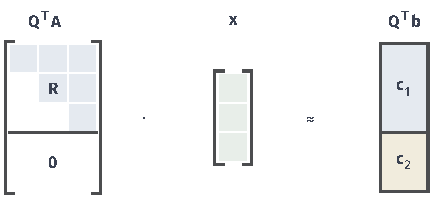
\includegraphics{figures/02-vectors-matrices-and-multivariate-calculus/03-linear-equations-and-optimization/tikz/learning-mechanisms/qr-residual-split.pdf}
  \caption{满列秩最小二乘的QR分解，示意$m=5,d=3$。正交变换后，矩阵上方的蓝色三角块为$\bm R$，下方为零；右端相应分成$\bm c_1$与$\bm c_2$。取$\bm R\hat{\bm x}=\bm c_1$后，残差$\bm r=\bm b-\bm A\hat{\bm x}$在变换后的坐标中上方为零，下方为$\bm c_2$，最小残差范数为$\lVert\bm c_2\rVert_2$。图中的近似号表示最小二乘匹配。}
  \label{fig:solver-qr-residual-split}
\end{figure}

\paragraph{满行秩的最小范数解}
同一种分解也能处理欠定方程。设$\bm A\in\mathbb R^{m\times d}$满行秩，$m<d$，求解目标改为第~\ref{sec:ls-select-among-solutions}节的最小范数精确解$\bm x_\star$。

最小范数解位于$\operatorname{range}(\bm A^\top)$中，需要的是这个子空间的标准正交基，所以对$\bm A^\top$而不是$\bm A$作薄QR分解
\begin{equation}
  \bm A^\top=\bm Q\bm R ,
 \label{eq:ls-qr-transpose-factorization}
\end{equation}
其中$\bm Q\in\mathbb R^{d\times m}$的列标准正交，$\bm R$为$m$阶可逆上三角矩阵。

于是
\[
  \bm A=\bm R^\top\bm Q^\top .
\]

把未知量写成$\bm x=\bm Q\bm y+\bm w$，其中$\bm Q^\top\bm w=\bm0$，代入方程得
\[
 \bm A\bm x=\bm R^\top\bm Q^\top\bm Q\bm y+\bm R^\top\bm Q^\top\bm w=\bm R^\top\bm y .
\]

方程只约束坐标$\bm y$，不约束$\bm w$。取$\bm w=\bm0$使范数最小（理由见算法分析），得
\begin{equation}
 \bm R^\top\bm y=\bm b,\qquad \bm x_\star=\bm Q\bm y .
 \label{eq:ls-qr-min-norm}
\end{equation}
第一式是下三角方程，按式~\eqref{eq:ls-forward-substitution}前代求出$\bm y$；第二式由坐标重建解。

\paragraph{只需应用正交因子}
两个分支都只用到$\bm Q^\top$或$\bm Q$对向量的作用，并不要求显式存出完整的$\bm Q$。后面三个小节提供三种计算方式：修正Gram--Schmidt直接算出$\bm Q_1$的各列，Householder方法保存一串反射向量，Givens方法保存一串旋转参数。它们都服务于上面同一个求解逻辑。

\subsection{算法实现}

输入是满列秩的$\bm A$与$\bm b$，输出是$\hat{\bm x}$；满行秩的欠定输入走本小节最后的转置QR分支。需要预先选定的只是因子的计算方法，三种选择见第~\ref{sec:ls-mgs}--\ref{sec:ls-givens}节。

算法由三个模块组成：QR分解给出$\bm R$并记录正交变换，变换右端求出$\bm c_1$，回代求出$\hat{\bm x}$。

下面仍用第~\ref{sec:ls-normal-equations-method}节的直线拟合数据逐步演示：
\[
  \bm A=\begin{bmatrix}1&0\\1&1\\1&2\end{bmatrix},\qquad \bm b=\begin{bmatrix}1\\2\\2\end{bmatrix}.
\]

\subsubsection{QR分解}
输入$\bm A$，输出$\bm R$以及正交因子或其变换记录。按第~\ref{sec:ls-mgs}、\ref{sec:ls-householder}、\ref{sec:ls-givens}节之一计算：修正Gram--Schmidt直接给出$\bm Q_1$的各列，Householder与Givens方法保存一串反射或旋转。

例中用修正Gram--Schmidt（逐步计算见第~\ref{sec:ls-mgs}节）得两个标准正交列
\[
 \bm q_1=\frac1{\sqrt3}\begin{bmatrix}1\\1\\1\end{bmatrix},\qquad
 \bm q_2=\frac1{\sqrt2}\begin{bmatrix}-1\\0\\1\end{bmatrix},
\]
以及三角因子
\[
 \bm R=\begin{bmatrix}\sqrt3&\sqrt3\\0&\sqrt2\end{bmatrix}.
\]

Householder与Givens方法给出的$\bm R$与它至多相差各行的符号。

若某个对角元$r_{j,j}=0$，说明$\bm A$秩亏，停止并改用第~\ref{sec:ls-svd-solve}节的SVD求解。

\subsubsection{变换右端}
输入正交因子与$\bm b$，输出$\bm c_1$。
\begin{enumerate}
 \item \textbf{计算$\bm c_1$。}按式~\eqref{eq:ls-qr-triangular-system}计算$\bm c_1=\bm Q_1^\top\bm b$。使用反射或旋转时，把它们按分解时的次序依次作用于$\bm b$，取结果的前$d$个分量；修正Gram--Schmidt中$\bm c_1$的计算次序在第~\ref{sec:ls-mgs}节说明。
 
 例中
 \[
  \bm c_1=\begin{bmatrix}\bm q_1^\top\bm b\\\bm q_2^\top\bm b\end{bmatrix}
  =\begin{bmatrix}5/\sqrt3\\1/\sqrt2\end{bmatrix}.
 \]

 \item \textbf{读出最小残差。}使用反射或旋转时，变换后右端的其余分量就是$\bm c_2$，$\lVert\bm c_2\rVert_2$即最小残差范数。
 
 例中若把$\bm Q_1$补齐为正交方阵，第三个标准正交向量及相应的右端分量为
 \[
  \bm q_3=\frac1{\sqrt6}\begin{bmatrix}1\\-2\\1\end{bmatrix},\qquad
  \bm c_2=\bm q_3^\top\bm b=-\frac1{\sqrt6},
 \]
 最小残差范数为$1/\sqrt6$。
\end{enumerate}

\subsubsection{回代}
输入$\bm R$与$\bm c_1$，输出$\hat{\bm x}$。
\begin{enumerate}
 \item \textbf{逐个求出$\hat x_i$。}根据式~\eqref{eq:ls-back-substitution}，对$i=d,\ldots,1$依次由式~\eqref{eq:ls-qr-triangular-system}得
 \[
  \hat x_i=\frac{(\bm c_1)_i-\sum_{j>i}r_{i,j}\hat x_j}{r_{i,i}} ;
 \]
 求出$\hat x_1$后结束。
 
 例中
 \[
  \hat x_2=\frac{1/\sqrt2}{\sqrt2}=\frac12,\qquad
  \hat x_1=\frac{\frac5{\sqrt3}-\sqrt3\cdot\frac12}{\sqrt3}=\frac76 .
 \]

 \item \textbf{输出并核验。}输出$\hat{\bm x}$，并以原始数据核验$\bm A^\top(\bm b-\bm A\hat{\bm x})=\bm0$。
 
 例中解与残差为
 \[
  \hat{\bm x}=\begin{bmatrix}7/6\\1/2\end{bmatrix},\qquad
  \bm r=\begin{bmatrix}-1/6\\1/3\\-1/6\end{bmatrix},
 \]
 并且$\bm A^\top\bm r=\bm0$。残差长度$1/\sqrt6$与上面读出的$\lvert\bm c_2\rvert$相同。
\end{enumerate}

例中的$\bm R$与$\bm c_1$恰是正规方程法中的$\bm L^\top$与前代结果$\bm y$：两条路线最后回代的是同一个三角方程，区别在于这里没有形成$\bm A^\top\bm A$。

\subsubsection{欠定情形：转置QR}
输入满行秩的$\bm A$（$m<d$）与$\bm b$，输出最小范数解$\bm x_\star$。
\begin{enumerate}
 \item \textbf{分解转置。}用上述任一种方法计算薄QR分解$\bm A^\top=\bm Q\bm R$。若$\bm R$出现零对角元，说明$\bm A$秩亏，停止并改用SVD求解。
 \item \textbf{前代。}根据式~\eqref{eq:ls-qr-min-norm}与式~\eqref{eq:ls-forward-substitution}，由下三角方程$\bm R^\top\bm y=\bm b$依次求出$y_1,\ldots,y_m$。
 \item \textbf{重建并核验。}计算$\bm x_\star=\bm Q\bm y$并输出，检查$\bm A\bm x_\star=\bm b$及$\bm x_\star\in\operatorname{range}(\bm A^\top)$。
\end{enumerate}

下例用一个欠定方程走一遍上述三步。

\begin{example}[转置QR给出最小范数解]
\label{ex:ls-qr-min-norm-run}
考虑下面的欠定方程：
\[
 \bm A=\begin{bmatrix}1&0&1\\0&1&1\end{bmatrix},\qquad
 \bm b=\begin{bmatrix}1\\2\end{bmatrix}.
\]
它有无穷多解。

$\bm A^\top$的两列为$(1,0,1)^\top$与$(0,1,1)^\top$。按修正Gram--Schmidt，先归一化第一列，并求出第二列沿它的分量：
\[
 \bm q_1=\frac1{\sqrt2}\begin{bmatrix}1\\0\\1\end{bmatrix},\qquad
 r_{1,2}=\frac1{\sqrt2}.
\]
扣除这一分量后归一化，得
\[
 \bm q_2=\frac1{\sqrt6}\begin{bmatrix}-1\\2\\1\end{bmatrix}.
\]
三角因子为
\[
 \bm R=\begin{bmatrix}\sqrt2&1/\sqrt2\\0&\sqrt{3/2}\end{bmatrix}.
\]
前代求解$\bm R^\top\bm y=\bm b$：
\[
 \begin{aligned}
 \sqrt2\,y_1&=1, & y_1&=\tfrac1{\sqrt2};\\
 \tfrac1{\sqrt2}y_1+\sqrt{3/2}\,y_2&=2, & y_2&=\sqrt{3/2} .
 \end{aligned}
\]
重建得
\[
 \bm x_\star=y_1\bm q_1+y_2\bm q_2
 =\frac12\begin{bmatrix}1\\0\\1\end{bmatrix}+\frac12\begin{bmatrix}-1\\2\\1\end{bmatrix}
 =\begin{bmatrix}0\\1\\1\end{bmatrix}.
\]
可以直接确认它的范数最小：本例全部解为$(1-t,2-t,t)^\top$，$t\in\mathbb R$，其范数平方为
\[
 (1-t)^2+(2-t)^2+t^2=3(t-1)^2+2 ,
\]
在$t=1$时最小，对应的正是$\bm x_\star$。
\end{example}

\subsection{算法分析}

\paragraph{正确性}
两个分支的正确性合写成下面的定理。

\begin{theorem}[QR给出最小二乘解与最小范数解]
\label{thm:ls-qr-least-squares}
设$\bm A\in\mathbb R^{m\times d}$，$\bm b\in\mathbb R^m$。
\begin{enumerate}
 \item 设$\bm A$满列秩，$\bm A=\bm Q\left[\begin{smallmatrix}\bm R\\\bm0\end{smallmatrix}\right]$，$\bm Q^\top\bm b=\left[\begin{smallmatrix}\bm c_1\\\bm c_2\end{smallmatrix}\right]$。则$\hat{\bm x}=\bm R^{-1}\bm c_1$是唯一的最小二乘解，最小残差范数为$\lVert\bm c_2\rVert_2$。
 \item 设$\bm A$满行秩，$\bm A^\top=\bm Q\bm R$为薄QR分解，$\bm R^\top\bm y=\bm b$。则$\bm x_\star=\bm Q\bm y$是$\bm A\bm x=\bm b$唯一的最小范数解。
\end{enumerate}
\end{theorem}
\begin{proof}
(1) 正交矩阵满足$\lVert\bm Q^\top\bm z\rVert_2^2=\bm z^\top\bm Q\bm Q^\top\bm z=\lVert\bm z\rVert_2^2$，所以式~\eqref{eq:ls-qr-residual-split}成立，其第二项与$\bm x$无关；$\bm R$可逆，第一项当且仅当$\bm x=\bm R^{-1}\bm c_1$时为零。

(2) 由$\bm Q^\top\bm Q=\bm I$，
\[
 \bm A\bm x_\star=\bm R^\top\bm Q^\top\bm Q\bm y=\bm R^\top\bm y=\bm b ,
\]
并且$\bm x_\star\in\operatorname{range}(\bm Q)=\operatorname{range}(\bm A^\top)=(\ker\bm A)^\perp$。任何其他解都与$\bm x_\star$相差$\ker\bm A$中的非零向量，即主要思想中的$\bm w\neq\bm0$，由勾股关系
\[
 \lVert\bm Q\bm y+\bm w\rVert_2^2=\lVert\bm y\rVert_2^2+\lVert\bm w\rVert_2^2 ,
\]
其范数更大。
\end{proof}

\paragraph{数值敏感度}
数值上要区分两个来源：最小二乘问题本身对数据的敏感度由问题决定（第~\ref{sec:ls-ls-regularization-sensitivity}节），计算QR因子时引入多少误差则取决于所用的正交化过程。三种实现在因子构造的工作量、数值正交性和残差核验方式上并不相同，下面分别说明。

\paragraph{秩亏情形}
秩亏时$\bm R$出现零对角元，不能照搬可逆$\bm R$的回代，最小范数最小二乘解按第~\ref{sec:ls-svd-solve}节用SVD求解。带列主元的QR能把线性无关的主元列排到前面，但只取主元变量回代、把其余原坐标置零，一般得到的是基本解，不能据此认定它是最小范数解。所以一般秩的情形本章统一使用SVD路线。

\subsection{修正Gram--Schmidt正交化}
\label{sec:ls-mgs}

本小节与后两小节计算同一组QR因子，思路分为两类。修正Gram--Schmidt从$\bm A$的各列出发，逐个造出标准正交方向，直接得到$\bm Q_1$的各列与$\bm R$。

Householder反射与Givens旋转则不写出$\bm Q$的列，而是对$\bm A$和$\bm b$依次施加正交变换，直到$\bm A$变成上三角形；正交因子只以这串变换的记录形式存在。正交变换保持长度，每一步之后$\lVert\bm A\bm x-\bm b\rVert_2$对任意$\bm x$都不变，所以变换结束时得到的正是式~\eqref{eq:ls-qr-triangular-system}的三角方程。

修正Gram--Schmidt的想法是一次确定一个新方向：一列减去它在已有方向上的分量，剩下的部分是这一列带来的新方向，归一化后就是下一个$\bm q_j$；减去的分量与剩下部分的长度记入$\bm R$。

\subsubsection{主要思想}
\term{修正Gram--Schmidt}（modified Gram--Schmidt）处理满列秩的$\bm A\in\mathbb R^{m\times d}$（$m\geq d$），目标是薄QR分解$\bm A=\bm Q_1\bm R$的因子。按列比较两边，第$k$列是
\begin{equation}
 \bm a_k=r_{1,k}\bm q_1+r_{2,k}\bm q_2+\cdots+r_{k,k}\bm q_k .
 \label{eq:ls-mgs-column-expansion}
\end{equation}
这个等式说明了$\bm R$中各元素的含义：$r_{i,k}$（$i<k$）是$\bm a_k$沿已有方向$\bm q_i$的分量，$r_{k,k}$是扣除这些分量后剩余部分的长度，$\bm q_k$是剩余部分的方向。$\bm R$是上三角矩阵，第$k$列只用到前$k$个方向，因此可以按列的次序逐个求出方向。

\paragraph{$d=2$的情况}
以$d=2$为例，两个等式是
\[
 \bm a_1=r_{1,1}\bm q_1,\qquad \bm a_2=r_{1,2}\bm q_1+r_{2,2}\bm q_2 .
\]
由第一式和$\lVert\bm q_1\rVert_2=1$，得
\[
 r_{1,1}=\lVert\bm a_1\rVert_2,\qquad \bm q_1=\bm a_1/r_{1,1} .
\]
第二式两边与$\bm q_1$作内积，由$\bm q_1^\top\bm q_2=0$得
\[
 r_{1,2}=\bm q_1^\top\bm a_2 ;
\]
移项后
\[
 r_{2,2}\bm q_2=\bm a_2-r_{1,2}\bm q_1 ,
\]
右边是$\bm a_2$扣除$\bm q_1$方向分量后的剩余向量，所以$r_{2,2}$是它的长度，$\bm q_2$是它的方向。

\paragraph{一般情况}
列数更多时，每一列要扣除的已有方向也更多。记$\bm v_k$为第$k$列的当前剩余向量，即第$k$列中尚未由已有方向表示的部分，开始时$\bm v_k=\bm a_k$。修正形式的做法是：每得到一个新方向，就立刻从所有尚未处理的列中扣除这一方向上的分量。于是轮到第$j$列时，$\bm v_j$已经扣除了$\bm q_1,\ldots,\bm q_{j-1}$方向的分量，剩下的只有新方向，由第$j$列的等式得
\begin{equation}
 r_{j,j}=\lVert\bm v_j\rVert_2,\qquad \bm q_j=\bm v_j/r_{j,j};
 \label{eq:ls-mgs-normalize}
\end{equation}
随后对每个$k>j$扣除$\bm q_j$方向的分量：
\begin{equation}
 r_{j,k}=\bm q_j^\top\bm v_k,\qquad \bm v_k\leftarrow\bm v_k-r_{j,k}\bm q_j .
 \label{eq:ls-mgs-update}
\end{equation}

与第~\ref{chap:inner-product-spaces}章的Gram--Schmidt正交化相比，它只差一处：投影系数用已经扣除了前面分量的当前剩余向量计算，而不是都用原始列$\bm a_k$。

精确算术中两种算法给出同一组因子。有限精度下，算出的$\bm q_2$与$\bm q_1$并不严格正交。原来的做法用$\bm q_2^\top\bm a_k$计算系数；若$\bm a_k$在$\bm q_1$方向上的分量很大，$\bm q_2$对正交性的微小偏离会与这一大分量相乘，混入$r_{2,k}$。

修正形式所用的$\bm v_k$已经扣除了$\bm q_1$方向的分量，同样的偏离只与很小的残留分量相乘。这只说明误差的来源，正交性的检查方法见本小节的算法分析。

求解还需要$\bm c_1=\bm Q_1^\top\bm b$。把右端当作额外的一列，按同样的次序扣除：令$\bm s=\bm b$，对$i=1,\ldots,d$依次计算
\begin{equation}
 c_i=\bm q_i^\top\bm s,\qquad \bm s\leftarrow\bm s-c_i\bm q_i .
 \label{eq:ls-mgs-rhs}
\end{equation}
每次扣除取走$\bm b$在一个方向上能由$\bm A$的列表示的部分，$c_i$记录取走的量。全部扣除后，$\bm s$就是$\bm b$减去它在列空间上的投影，即最小二乘残差；$\bm c_1=(c_1,\ldots,c_d)^\top$交给式~\eqref{eq:ls-qr-triangular-system}回代。

\subsubsection{算法实现}
输入是满列秩的$\bm A$与$\bm b$，输出是$\hat{\bm x}$，没有需要预先选定的规则。算法逐列进行，用$j$记当前处理的列，维护剩余向量$\bm v_1,\ldots,\bm v_d$、$\bm R$的已算元素和右端的剩余向量$\bm s$；全部列处理完后回代。

下面仍用直线拟合数据逐步演示：
\[
  \bm A=\begin{bmatrix}1&0\\1&1\\1&2\end{bmatrix},\qquad \bm b=\begin{bmatrix}1\\2\\2\end{bmatrix}.
\]

\begin{enumerate}
 \item \textbf{初始化。}令$\bm v_k=\bm a_k$（$k=1,\ldots,d$），$\bm R=\bm0$，$\bm s=\bm b$，$j=1$。

 例中两列的剩余向量为
 \[
  \bm v_1=\begin{bmatrix}1\\1\\1\end{bmatrix},\qquad
  \bm v_2=\begin{bmatrix}0\\1\\2\end{bmatrix},
 \]
 右端的剩余向量为$\bm s=(1,2,2)^\top$。

 \item \textbf{归一化当前列。}此时$\bm v_j$已经扣除了全部已有方向的分量，剩下的是第$j$列带来的新方向。根据式~\eqref{eq:ls-mgs-normalize}算出它的长度$r_{j,j}$与方向$\bm q_j$。若$r_{j,j}=0$，说明第$j$列落在前面各列的张成中，满列秩的前提不成立，停止并改用SVD求解。

 例中$j=1$，
 \[
  r_{1,1}=\lVert\bm v_1\rVert_2=\sqrt3,\qquad
  \bm q_1=\frac1{\sqrt3}\begin{bmatrix}1\\1\\1\end{bmatrix}.
 \]

 \item \textbf{扣除新方向。}新方向一经确定，就从后面各列和右端中扣除，后续步骤面对的都是已经扣除这一方向的向量。根据式~\eqref{eq:ls-mgs-update}，对每个$k>j$算出$r_{j,k}$并更新$\bm v_k$；再根据式~\eqref{eq:ls-mgs-rhs}算出$c_j$并更新$\bm s$。

 例中对第二列，先求分量$r_{1,2}=\bm q_1^\top\bm v_2=\sqrt3$，再扣除：
 \[
  \bm v_2\leftarrow\begin{bmatrix}0\\1\\2\end{bmatrix}-\begin{bmatrix}1\\1\\1\end{bmatrix}=\begin{bmatrix}-1\\0\\1\end{bmatrix}.
 \]
 对右端，先求$c_1=\bm q_1^\top\bm s=5/\sqrt3$，再扣除：
 \[
  \bm s\leftarrow\begin{bmatrix}1\\2\\2\end{bmatrix}-\frac53\begin{bmatrix}1\\1\\1\end{bmatrix}=\begin{bmatrix}-2/3\\1/3\\1/3\end{bmatrix}.
 \]

 在直线拟合中，扣除全一方向$\bm q_1$就是减去平均值：$\bm v_2$是横坐标$0,1,2$减去均值$1$，$\bm s$是$\bm b$减去均值$5/3$。

 \item \textbf{判断是否结束。}若$j<d$，令$j\leftarrow j+1$，回到第2步；否则结束。

 例中$j=1<2$，令$j=2$。第2步得
 \[
  r_{2,2}=\lVert\bm v_2\rVert_2=\sqrt2,\qquad
  \bm q_2=\frac1{\sqrt2}\begin{bmatrix}-1\\0\\1\end{bmatrix};
 \]
 第3步右侧已没有待处理的列，只处理右端：先求$c_2=\bm q_2^\top\bm s=1/\sqrt2$，再扣除，
 \[
  \bm s\leftarrow\begin{bmatrix}-2/3\\1/3\\1/3\end{bmatrix}-\frac12\begin{bmatrix}-1\\0\\1\end{bmatrix}=\begin{bmatrix}-1/6\\1/3\\-1/6\end{bmatrix}.
 \]

 这时$j=d$，结束，得
 \[
  \bm R=\begin{bmatrix}\sqrt3&\sqrt3\\0&\sqrt2\end{bmatrix},\qquad
  \bm c_1=\begin{bmatrix}5/\sqrt3\\1/\sqrt2\end{bmatrix}.
 \]
 可以核验
 \[
  \bm q_1^\top\bm q_2=0,\qquad
  \sqrt3\,\bm q_1+\sqrt2\,\bm q_2=\begin{bmatrix}0\\1\\2\end{bmatrix}=\bm a_2 .
 \]
 第二式正是$\bm R$第二列的含义：$\bm a_2$沿$\bm q_1$的分量为$\sqrt3$，剩余部分长度为$\sqrt2$。

 最后剩下的$\bm s$正是直线拟合的残差，长度为$1/\sqrt6$。

 \item \textbf{回代。}按式~\eqref{eq:ls-qr-triangular-system}回代求解$\bm R\hat{\bm x}=\bm c_1$，输出$\hat{\bm x}$。

 例中的$\bm R$与$\bm c_1$与第~\ref{sec:ls-qr-method}节算法实现所用的相同，回代得
 \[
  \hat{\bm x}=\begin{bmatrix}7/6\\1/2\end{bmatrix}.
 \]
\end{enumerate}

$\bm Q_1$、$\bm R$和剩余向量都只是内部状态。按列组织时也可以对第$j$列依次扣除$\bm q_1,\ldots,\bm q_{j-1}$方向的分量，每次内积都用刚更新过的剩余向量；它对每一列执行的运算与上面相同，只是循环次序不同。

有限精度下若发现某列扣除后明显变短，可以对它再正交化一遍，并把第二遍得到的投影系数加到已累计的$r_{i,j}$上，使$\bm A=\bm Q_1\bm R$仍然成立。右端也要按式~\eqref{eq:ls-mgs-rhs}逐次扣除：有限精度下$\bm Q_1$的列不完全正交，不宜把它换成另算$\bm Q_1^\top\bm b$。

\subsubsection{算法分析}
先看精确算术中的不变关系。式~\eqref{eq:ls-mgs-update}更新后，
\[
  \bm q_j^\top\bm v_k=\bm q_j^\top\bm v_k-r_{j,k}=0 ,
\]
即$\bm v_k$与$\bm q_j$正交。

扣除的是$\bm q_j$方向的分量，而$\bm q_j$与$\bm q_1,\ldots,\bm q_{j-1}$正交，所以$\bm v_k$仍与它们正交。因此第$j$步归一化的$\bm v_j$与此前全部方向正交，各$\bm q_i$两两正交。

同时，每次扣除都把分量记入$\bm R$，所以整个过程维持
\begin{equation}
 \bm a_k=\sum_{i\leq j}r_{i,k}\bm q_i+\bm v_k\qquad(k>j),
 \label{eq:ls-mgs-invariant}
\end{equation}
即原始列始终等于已提取的分量加上当前剩余向量。

全部列处理完毕时剩余部分已归入各$\bm q_k$，得到
\[
  \bm A=\bm Q_1\bm R .
\]

又因各$\bm q_i$两两正交，对剩余向量和对原始列计算的内积相同：
\begin{equation}
  \bm q_i^\top\Bigl(\bm a_j-\sum_{k<i}r_{k,j}\bm q_k\Bigr)=\bm q_i^\top\bm a_j .
 \label{eq:ls-mgs-cgs-equivalence}
\end{equation}

所以修正形式给出与原来相同的QR分解；同样的论证说明式~\eqref{eq:ls-mgs-rhs}给出$c_i=\bm q_i^\top\bm b$。由定理~\ref{thm:ls-qr-least-squares}，回代所得即最小二乘解。

有限精度下，近相关的列扣除旧方向后剩余向量很短，其中舍入误差的相对影响被放大，算出的$\bm q_j$会偏离正交，这就是再正交化要处理的情形。

检查结果时用$\lVert\bm Q_1^\top\bm Q_1-\bm I\rVert$衡量正交性，用$\lVert\bm A-\bm Q_1\bm R\rVert$衡量重构质量，二者要分开看：后者小并不保证前者小。正交性损失的程度与$\bm A$的条件数有关，具体说明见第~\ref{sec:ls-numerical-stability}节。主要工作约为$2md^2$次运算。

\subsection{Householder反射}
\label{sec:ls-householder}

\subsubsection{主要思想}
Householder方法不构造$\bm Q_1$的列，而是逐列把$\bm A$化成上三角形。第$k$步用一个镜面反射，把第$k$列从对角元往下的部分变成坐标轴方向，于是对角元下方的元素全部变为零；同一个反射也作用于其余各列和$\bm b$。

$d$次反射之后得到$\bm R$与变换后的右端，正交因子就是这一串反射的乘积：
\begin{equation}
  \bm Q^\top=\bm H_d\cdots\bm H_1
 \label{eq:ls-householder-qt}
\end{equation}
使$\bm H_d\cdots\bm H_1\bm A$成为上三角矩阵。

第$k$步的核心问题是：给定一个列段$\bm y\neq\bm0$，怎样构造正交矩阵把它映到第一个坐标轴上。

正交变换不改变长度，$\bm y$只能被送到同样长的轴向量$\alpha\bm e_1$，$\lvert\alpha\rvert=\lVert\bm y\rVert_2$。在平面上可以直接找到这样的变换：$\bm y$与$\alpha\bm e_1$到原点的距离相同，原点落在两点连线的垂直平分线上；以这条垂直平分线为镜子作反射，$\bm y$恰好落到$\alpha\bm e_1$。镜子与两点之差$\bm y-\alpha\bm e_1$垂直，所以镜子的法向就是$\bm v=\bm y-\alpha\bm e_1$。高维时镜子换成以$\bm v$为法向的超平面。

这种反射称为\term{Householder反射}（Householder reflection），写作
\begin{equation}
  \bm H=\bm I-2\bm v\bm v^\top/(\bm v^\top\bm v)
 \label{eq:ls-householder-reflector}
\end{equation}
它把$\bm v$方向的分量变号，保持与$\bm v$正交的分量不变，是关于以$\bm v$为法向的超平面的镜面反射。它对称且正交，所以只需选好$\bm v$，如图~\ref{fig:ls-householder-reflection}所示。

\begin{figure}[htbp]
  \centering
  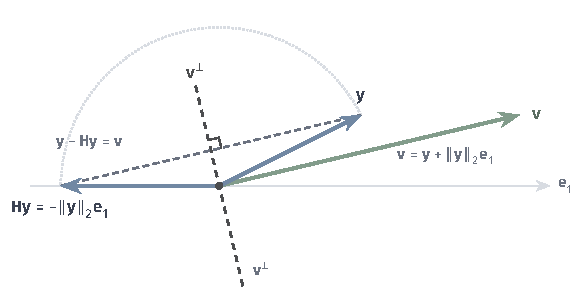
\includegraphics[width=98.94mm]{figures/01-basic-mathematics/03-vectors-matrices-and-multivariate-functions/tikz/c5-householder-reflection/figure.pdf}
  \caption{Householder反射的几何。取$\bm y=(2,1)^\top$，按式~\eqref{eq:ls-householder}令$\bm v=\bm y+\sqrt5\,\bm e_1$。反射超平面$\bm v^\perp$是$\bm y$与$\bm H\bm y=-\sqrt5\,\bm e_1$连线的垂直平分线，两者之差恰为$\bm v$；点线圆弧表示反射保持长度。解析式构造。}
  \label{fig:ls-householder-reflection}
\end{figure}

几何构造给出的$\bm v$也可以从代数上确认。要求的等式是$\bm H\bm y=\alpha\bm e_1$。正交变换保持长度，所以
\[
 \alpha^2=\bm y^\top\bm y,\qquad \alpha=\pm\lVert\bm y\rVert_2 .
\]
展开左边，
\[
 \bm H\bm y=\bm y-\frac{2\bm v^\top\bm y}{\bm v^\top\bm v}\,\bm v=\alpha\bm e_1 ,
\]
所以$\bm y-\alpha\bm e_1$必须是$\bm v$的倍数。反射只依赖$\bm v$的方向，于是取
\[
 \bm v=\bm y-\alpha\bm e_1 ;
\]
这一选择确实使系数$2\bm v^\top\bm y/(\bm v^\top\bm v)$等于$1$，从而
\[
 \bm H\bm y=\bm y-\bm v=\alpha\bm e_1 ,
\]
验证见本小节算法分析中的引理。

$\alpha$的两个符号对应坐标轴上的两个候选目标$\pm\lVert\bm y\rVert_2\bm e_1$，精确算术中都可以用。若$\bm y$本来就接近其中一个目标，它与该目标几乎重合，二者之差$\bm v$很短，镜子的朝向难以准确算出；所以实际选择与$\bm y$的首分量异号、离$\bm y$较远的那个目标。具体地取$\alpha=-s\lVert\bm y\rVert_2$，其中$y_1\geq0$时$s=1$、$y_1<0$时$s=-1$，即
\begin{equation}
 \bm v=\bm y+s\lVert\bm y\rVert_2\bm e_1,\qquad
 \bm H=\bm I-\frac{2\bm v\bm v^\top}{\bm v^\top\bm v},
 \label{eq:ls-householder}
\end{equation}
这样$\bm v$的首分量$v_1=y_1+s\lVert\bm y\rVert_2$是两个同号数相加；数值上的理由见算法分析。

作用于其他向量时不形成稠密的$\bm H$：令$\tau=2/(\bm v^\top\bm v)$，则对任意向量$\bm z$都有
\begin{equation}
 \bm H\bm z=\bm z-\tau\,(\bm v^\top\bm z)\,\bm v ,
 \label{eq:ls-householder-apply}
\end{equation}
即减去$\bm z$在$\bm v$方向上分量的两倍，只需一次内积和一次向量更新。

第$k$步的反射只作用于第$k$至$m$行，嵌入$m$阶后为
\begin{equation}
 \bm H_k=\operatorname{diag}(\bm I_{k-1},\bm H) .
 \label{eq:ls-householder-embedding}
\end{equation}
前$k-1$行已经是$\bm R$的确定部分，不再改动；前$k-1$列在第$k$至$m$行上的零也保持为零（见算法分析），所以逐列进行时，已经造出的零不会被后面的反射破坏。

\subsubsection{算法实现}
输入是满列秩的$\bm A\in\mathbb R^{m\times d}$（$m\geq d$）与$\bm b$，输出是$\hat{\bm x}$。需要预先选定的规则是式~\eqref{eq:ls-householder}中符号$s$的取法，并保持原列顺序，不选列主元。

算法逐列进行，用$k$记当前处理的列，维护工作矩阵$\bm F$与工作右端$\bm c$；三角化结束后回代。仍用直线拟合数据演示，每一列处理完后给出$\bm F$与$\bm c$的当前值。
\begin{enumerate}
 \item \textbf{初始化。}令$\bm F=\bm A$，$\bm c=\bm b$，$k=1$。

 例中
 \[
  \bm F=\begin{bmatrix}1&0\\1&1\\1&2\end{bmatrix},\qquad
  \bm c=\begin{bmatrix}1\\2\\2\end{bmatrix}.
 \]

 \item \textbf{构造反射。}取当前列段$\bm y=\bm F_{k:m,k}$，即第$k$列中从对角元往下、尚未处理的部分，根据式~\eqref{eq:ls-householder}构造$\bm v$与$\tau=2/(\bm v^\top\bm v)$，保存这一反射记录。
 
 若$\bm y=\bm0$，说明第$k$列落在前面各列的张成中，满列秩的前提不成立，停止并改用SVD求解；若$\bm y$在第一个分量以下已经全为零，可以取恒等变换，跳过第3步。

 例中$k=1$，$\bm y=(1,1,1)^\top$，$\lVert\bm y\rVert_2=\sqrt3$，$y_1>0$，取$s=1$，于是
 \[
  \bm v=\begin{bmatrix}1+\sqrt3\\1\\1\end{bmatrix},\qquad \bm v^\top\bm v=6+2\sqrt3,\qquad \tau=\frac1{3+\sqrt3}.
 \]

 \item \textbf{作用于剩余子块与右端。}整个问题必须经受同一个正交变换，残差长度才保持不变，所以反射不仅作用于第$k$列，也作用于其余各列和右端。
 
 根据式~\eqref{eq:ls-householder-apply}，把这个反射作用于剩余子块$\bm F_{k:m,k:d}$的各列和右端$\bm c_{k:m}$；第$k$列不必计算，直接成为$(-s\lVert\bm y\rVert_2,0,\ldots,0)^\top$。

 例中第一列变为$(-\sqrt3,0,0)^\top$；对第二列$\bm z=(0,1,2)^\top$与右端$\bm c$分别算出
 \[
  \begin{aligned}
  &\text{第二列：}&& \bm v^\top\bm z=3,\quad \tau\,\bm v^\top\bm z=\tfrac{3-\sqrt3}2;\\
  &\text{右端：}&& \bm v^\top\bm c=5+\sqrt3,\quad \tau\,\bm v^\top\bm c=2-\tfrac{\sqrt3}3 .
  \end{aligned}
 \]
 各自减去相应倍数的$\bm v$，得
 \[
  \bm F=\begin{bmatrix}-\sqrt3&-\sqrt3\\0&\frac{\sqrt3-1}2\\[2pt]0&\frac{\sqrt3+1}2\end{bmatrix},\qquad
  \bm c=\begin{bmatrix}-5/\sqrt3\\1/\sqrt3\\1/\sqrt3\end{bmatrix}.
 \]
 第一列已经成为坐标轴方向，第一行从此确定，后面只处理第2、3行。两列与右端的长度平方仍为$3$、$5$、$9$，与变换前相同，这是反射保持长度的直接检验。

 \item \textbf{判断是否结束。}若$k<d$，令$k\leftarrow k+1$，回到第2步；否则结束。

 例中$k=1<2$，令$k=2$。第2步取第二列的后两个元素
 \[
  \bm y=\begin{bmatrix}\frac{\sqrt3-1}2\\[2pt]\frac{\sqrt3+1}2\end{bmatrix},\qquad
  \lVert\bm y\rVert_2=\sqrt2,\qquad s=1,
 \]
 由此构造反射向量
 \[
  \bm v=\begin{bmatrix}\frac{\sqrt3-1}2+\sqrt2\\[2pt]\frac{\sqrt3+1}2\end{bmatrix}.
 \]
 第3步只作用于后两行，第二列的这一段与右端的后两个分量分别变为
 \[
  \begin{bmatrix}-\sqrt2\\0\end{bmatrix},\qquad
  \begin{bmatrix}-1/\sqrt2\\-1/\sqrt6\end{bmatrix}.
 \]
 这一段也成为坐标轴方向，第一列的零与第一行都没有改动。

 这时$k=d$，结束，得
 \[
  \bm F=\begin{bmatrix}-\sqrt3&-\sqrt3\\0&-\sqrt2\\0&0\end{bmatrix},\qquad
  \bm c=\begin{bmatrix}-5/\sqrt3\\-1/\sqrt2\\-1/\sqrt6\end{bmatrix}.
 \]

 \item \textbf{回代。}取$\bm R=\bm F_{1:d,1:d}$，检查对角元非零，再按式~\eqref{eq:ls-qr-triangular-system}回代求解$\bm R\hat{\bm x}=\bm c_{1:d}$，输出$\hat{\bm x}$；$\bm F$的后$m-d$行为零，$\bm c_{d+1:m}$是任何$\bm x$都无法拟合的部分，$\lVert\bm c_{d+1:m}\rVert_2$是最小残差范数。

 例中
 \[
  \hat x_2=\frac{-1/\sqrt2}{-\sqrt2}=\frac12,\qquad
  \hat x_1=\frac{-\frac5{\sqrt3}+\sqrt3\cdot\frac12}{-\sqrt3}=\frac53-\frac12=\frac76,
 \]
 $\lvert c_3\rvert=1/\sqrt6$正是最小残差范数。
\end{enumerate}

例中的$\bm R$与正规方程法的Cholesky因子$\bm L^\top$只差各行的符号。对角元为负不影响求解；若要统一成正对角，须把$\bm R$的相应行与变换后右端的相应分量同时变号。

\subsubsection{算法分析}
单步消元的依据是下面的引理。

\begin{lemma}[Householder反射]
\label{lem:ls-householder-reflection}
设$\bm y\neq\bm0$，$\bm v$与$\bm H$由式~\eqref{eq:ls-householder}给出。则$\bm H$对称正交，且$\bm H\bm y=-s\lVert\bm y\rVert_2\bm e_1$。
\end{lemma}
\begin{proof}
$\bm H$显然对称；
\[
 \bm H^2=\bm I-\frac{4\bm v\bm v^\top}{\bm v^\top\bm v}+\frac{4\bm v(\bm v^\top\bm v)\bm v^\top}{(\bm v^\top\bm v)^2}=\bm I ,
\]
所以$\bm H^\top\bm H=\bm I$。由$s^2=1$与$sy_1=\lvert y_1\rvert$，
\[
 \bm v^\top\bm v=2\lVert\bm y\rVert_2^2+2\lVert\bm y\rVert_2\lvert y_1\rvert=2\bm v^\top\bm y>0,
\]
于是$\bm H\bm y=\bm y-\bm v=-s\lVert\bm y\rVert_2\bm e_1$。
\end{proof}

每个$\bm H_k$只作用于第$k$至$m$行；前$k-1$列在这些行上已经是零，反射后仍为零。所以旧的零结构保持不变，$d$步后$\bm F=\bm H_d\cdots\bm H_1\bm A$是上三角矩阵，$\bm c=\bm H_d\cdots\bm H_1\bm b$。这正是取$\bm Q^\top=\bm H_d\cdots\bm H_1$的QR分解，由定理~\ref{thm:ls-qr-least-squares}，回代所得即最小二乘解。

符号的选择影响数值精度。$\bm v$的首分量是$y_1-\alpha$；若$\alpha$与$y_1$同号且$\bm y$接近$\bm e_1$方向，这是两个相近数相减，会严重相消。取$\alpha=-s\lVert\bm y\rVert_2$使$v_1$成为两个同号数相加，避免了这种相消。

Householder QR后向稳定（第~\ref{sec:ls-numerical-stability}节），算出的$\bm Q$在舍入误差范围内保持正交，主要工作约为$2md^2-\tfrac23d^3$次运算。列主元可以辅助辨认近相关的列，但秩亏时的最小范数选择仍回到第~\ref{sec:ls-svd-solve}节。

\subsection{Givens旋转}
\label{sec:ls-givens}

Givens方法同样用正交变换把$\bm A$和$\bm b$化成上三角形，但每次只消去一个元素：在两行构成的平面内作一次旋转，把其中一个元素转为零。

Householder反射一步处理一整列，Givens旋转一步只改动两行，其余各行原样保留。当对角线以下只有少数非零元，或者要在已有的$\bm R$上补入一条新观测时，只需对少数几对行作旋转，这种局部性就带来实际的节省。

\subsubsection{主要思想}
\term{Givens旋转}（Givens rotation）在两个坐标构成的平面内旋转，其余坐标不变；每次只混合两行，消去其中一个元素。所求的正交因子$\bm Q^\top$是一串这样的旋转之积。图~\ref{fig:ls-givens-householder-elimination}把旋转与反射并置。

\begin{figure*}[htbp]
  \centering
  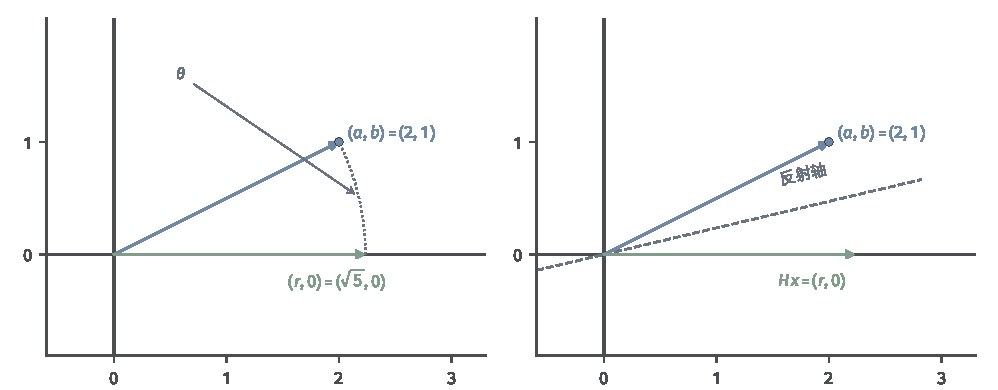
\includegraphics[width=168.998mm]{figures/00-shared/mathematical-preliminaries-upper/02-linear-spaces/matplotlib/ls-givens-householder-elimination/ls-givens-householder-elimination.pdf}
  \caption{两种初等正交消元。左：Givens旋转把$(a,b)=(2,1)^\top$沿圆弧旋到
  $(r,0)^\top$，$r=\sqrt5$，旋转角$\theta=\arctan(1/2)$；右：Householder反射沿角平分线
  把同一向量映到$(r,0)^\top$。两者都是正交变换，保持长度，区别在旋转（行列式$+1$）与
  反射（对称正交）。图中的反射取与式~\eqref{eq:ls-householder}相反的符号，精确算术中两种选择都可以。解析式教学构造。}
  \label{fig:ls-givens-householder-elimination}
\end{figure*}

先看二维问题：给定$(\alpha,\beta)^\top\neq\bm0$，求旋转$\bm G=\left[\begin{smallmatrix}c&s\\-s&c\end{smallmatrix}\right]$使$\bm G(\alpha,\beta)^\top=(\rho,0)^\top$。几何上，设向量$(\alpha,\beta)^\top$与第一坐标轴的夹角为$\theta$，把它顺时针转过$\theta$就落到第一坐标轴上；旋转保持长度，所以落点是$(\rho,0)^\top$，$\rho$是向量的长度。这个旋转矩阵的元素是$c=\cos\theta$与$s=\sin\theta$，而夹角的余弦与正弦就是$\alpha/\rho$与$\beta/\rho$，所以不必求出角度本身。

代数上逐个分量写出，连同旋转的条件，要求
\[
 c\alpha+s\beta=\rho,\qquad -s\alpha+c\beta=0,\qquad c^2+s^2=1 .
\]
由第二式，$(c,s)$与$(\alpha,\beta)$平行；由第三式归一化并取$\rho>0$，得
\[
 c=\frac\alpha\rho,\qquad s=\frac\beta\rho ;
\]
代入第一式得
\[
 \rho=\frac{\alpha^2+\beta^2}{\rho} .
\]
合起来，
\begin{equation}
 \begin{gathered}
 \rho=\sqrt{\alpha^2+\beta^2},\qquad c=\alpha/\rho,\qquad s=\beta/\rho,\\
 \bm G=\begin{bmatrix}c&s\\-s&c\end{bmatrix}.
 \end{gathered}
 \label{eq:ls-givens}
\end{equation}
这里的$s$与Householder反射中的符号无关。$\alpha=\beta=0$时取恒等变换。

对矩阵的两行$p,q$同时作用时，新的两行是
\begin{equation}
 \begin{aligned}
 \text{第}p\text{行}&\leftarrow c\cdot(\text{第}p\text{行})+s\cdot(\text{第}q\text{行}),\\
 \text{第}q\text{行}&\leftarrow -s\cdot(\text{第}p\text{行})+c\cdot(\text{第}q\text{行}),
 \end{aligned}
 \label{eq:ls-givens-rows}
\end{equation}
右端的两个分量也按同样的方式更新。参数$c,s$由两行在某一列的元素确定，使第$q$行在该列变为零、第$p$行在该列变为$\rho$；同一个旋转作用于两行的其余元素和右端，保证整个问题经受同一个正交变换。

三角化时逐列进行，在每一列中自下而上用相邻两行消去对角线下方的元素。每次旋转把下一行在这一列的元素并入上一行，非零部分就逐行向上汇集，最后集中到对角元上，对角元的绝对值等于这一列对角元及其下方各元素组成的列段的长度。被消零的行不再参与本列后面的旋转，前面各列的零也不受影响，理由见本小节的算法分析。

\subsubsection{算法实现}
输入是满列秩的$\bm A\in\mathbb R^{m\times d}$（$m\geq d$）和$\bm b$，输出是$\hat{\bm x}$。需要预先选定的规则是消元次序：按$k=1,\ldots,d$处理各列，在第$k$列中按$i=m,m-1,\ldots,k+1$自下而上消去$f_{i,k}$，每次使用相邻的第$i-1$、$i$两行。算法维护工作矩阵$\bm F$与工作右端$\bm t$，右端记作$\bm t$是为了不与旋转参数$c$混淆。下面先给出三角化与回代，再给出新增一条观测时的更新。仍用直线拟合数据演示，把右端写在增广列中。

\paragraph{三角化与回代}
\begin{enumerate}
 \item \textbf{初始化。}令$\bm F=\bm A$，$\bm t=\bm b$，$k=1$，$i=m$。

 例中
 \[
  [\bm F\mid\bm t]=\left[\begin{array}{cc|c}1&0&1\\1&1&2\\1&2&2\end{array}\right].
 \]

 \item \textbf{构造旋转。}若$f_{i,k}=0$，这个位置已经是零，直接转到第4步；否则令$\alpha=f_{i-1,k}$为上一行的元素、$\beta=f_{i,k}$为要消去的元素，根据式~\eqref{eq:ls-givens}计算$\rho,c,s$。为避免上溢或下溢，平方和可以先除以$\max(\lvert\alpha\rvert,\lvert\beta\rvert)$，开方后再恢复尺度，许多程序库以hypot函数提供这一计算。

 例中$k=1$、$i=3$，
 \[
  \alpha=\beta=1,\qquad \rho=\sqrt2,\qquad c=s=\frac1{\sqrt2}.
 \]

 \item \textbf{旋转两行。}根据式~\eqref{eq:ls-givens-rows}，用同一个$\bm G$作用于$\bm F$的第$i-1$、$i$两行在第$k$列及以后的部分，并同步变换$(t_{i-1},t_i)^\top$，保存这次旋转的参数。第$k$列以前的部分在两行中都是零，旋转后仍为零，不必计算。两式必须读取同一对旧行，计算时先用临时量保存旧值；若先覆盖第$i-1$行再用它计算第$i$行，结果就不再是旋转。

 例中第$2$、$3$两行变为
 \[
  \bigl(\sqrt2,\tfrac3{\sqrt2}\bigm|2\sqrt2\bigr),\qquad
  \bigl(0,\tfrac1{\sqrt2}\bigm|0\bigr).
 \]
 第3行的第一个元素已经消去，它的值并入第2行，第2行的首元素变为两个$1$组成的向量的长度$\sqrt2$。

 \item \textbf{判断是否结束。}若$i>k+1$，令$i\leftarrow i-1$，回到第2步；否则第$k$列已经完成，若$k<d$，令$k\leftarrow k+1$、$i=m$，回到第2步；若$k=d$，三角化结束。

 例中先令$i=2$，用第$1$、$2$行消去$f_{2,1}=\sqrt2$：
 \[
  \alpha=1,\qquad \beta=\sqrt2,\qquad \rho=\sqrt3,\qquad c=\frac1{\sqrt3},\qquad s=\sqrt{2/3},
 \]
 两行变为
 \[
  \bigl(\sqrt3,\sqrt3\bigm|\tfrac5{\sqrt3}\bigr),\qquad
  \bigl(0,\sqrt{3/2}\bigm|\sqrt{2/3}\bigr).
 \]
 第一列完成：三个$1$逐行向上汇集，对角元成为$\sqrt3=\lVert\bm a_1\rVert_2$。

 再令$k=2$、$i=3$，用第$2$、$3$行消去$f_{3,2}=1/\sqrt2$：
 \[
  \alpha=\sqrt{3/2},\qquad \beta=\frac1{\sqrt2},\qquad \rho=\sqrt2,\qquad c=\frac{\sqrt3}2,\qquad s=\frac12,
 \]
 两行变为
 \[
  \bigl(0,\sqrt2\bigm|\tfrac1{\sqrt2}\bigr),\qquad
  \bigl(0,0\bigm|-\tfrac1{\sqrt6}\bigr).
 \]
 这时$k=d$，结束，得
 \[
  [\bm F\mid\bm t]=\left[\begin{array}{cc|c}\sqrt3&\sqrt3&5/\sqrt3\\0&\sqrt2&1/\sqrt2\\0&0&-1/\sqrt6\end{array}\right].
 \]

 \item \textbf{回代。}取$\bm R=\bm F_{1:d,1:d}$，按式~\eqref{eq:ls-qr-triangular-system}回代求解$\bm R\hat{\bm x}=\bm t_{1:d}$，输出$\hat{\bm x}$，并用原始数据检查残差。

 例中$\bm R$恰为正规方程法的Cholesky因子$\bm L^\top$，$\bm t_{1:2}$恰为那里的前代结果$\bm y$，回代得
 \[
  \hat{\bm x}=\begin{bmatrix}7/6\\1/2\end{bmatrix},\qquad
  \lvert t_3\rvert=\frac1{\sqrt6},
 \]
 后者为最小残差范数。
\end{enumerate}

\paragraph{新增观测的更新}
局部消元的好处在新增观测时最明显。设已经有$d$阶上三角的$\bm R$和$\bm c_1$，新到一条观测行$\bm w^\top$及其右端$\eta$，要求加入这条观测后的最小二乘解，而不重新处理旧的观测行。

由式~\eqref{eq:ls-qr-residual-split}，旧观测对$\bm x$的全部约束都已经由$\lVert\bm R\bm x-\bm c_1\rVert_2^2$表达，$\lVert\bm c_2\rVert_2^2$只是与$\bm x$无关的常数。所以只需把新行排在$[\bm R\mid\bm c_1]$下方，再用旋转把它逐个元素并入$\bm R$。
\begin{enumerate}
 \item \textbf{排列。}把$(\bm w^\top\mid\eta)$排在$[\bm R\mid\bm c_1]$下方。例中在直线拟合的三个点之外新增点$(3,3)$，即$\bm w=(1,3)^\top$、$\eta=3$，上方是三角化得到的$\bm R$与$\bm c_1$，排列后为
 \[
  \left[\begin{array}{cc|c}\sqrt3&\sqrt3&5/\sqrt3\\0&\sqrt2&1/\sqrt2\\\hline1&3&3\end{array}\right].
 \]

 \item \textbf{逐个消去新行的元素。}对$k=1,\ldots,d$，取$\alpha=r_{k,k}$、$\beta$为新行当前的第$k$个元素，按式~\eqref{eq:ls-givens}与式~\eqref{eq:ls-givens-rows}旋转$\bm R$的第$k$行与新行，同时旋转$\bm c_1$的第$k$个分量与新右端；处理完$k=d$后新行全为零，结束。$\bm R$的第$k$行在前$k-1$列上是零，新行在这些列上也已消去，所以每次旋转都不会破坏已有的零。

 例中$k=1$时
 \[
  \alpha=\sqrt3,\qquad \beta=1,\qquad \rho=2,\qquad c=\frac{\sqrt3}2,\qquad s=\frac12,
 \]
 两行变为
 \[
  (2,3\mid4),\qquad \bigl(0,\sqrt3\bigm|\tfrac2{\sqrt3}\bigr);
 \]
 $k=2$时
 \[
  \alpha=\sqrt2,\qquad \beta=\sqrt3,\qquad \rho=\sqrt5,\qquad c=\sqrt{2/5},\qquad s=\sqrt{3/5},
 \]
 两行变为
 \[
  \bigl(0,\sqrt5\bigm|\tfrac3{\sqrt5}\bigr),\qquad \bigl(0,0\bigm|\tfrac1{\sqrt{30}}\bigr).
 \]
 新行的系数部分已经全部并入$\bm R$，右端剩下的$1/\sqrt{30}$是这条新观测带来的新增不可拟合部分。

 \item \textbf{回代。}用更新后的$\bm R$与$\bm c_1$回代，输出新的$\hat{\bm x}$。

 例中
 \[
  \bm R=\begin{bmatrix}2&3\\0&\sqrt5\end{bmatrix},\qquad
  \bm c_1=\begin{bmatrix}4\\3/\sqrt5\end{bmatrix},
 \]
 回代得
 \[
  \hat x_2=\frac{3/\sqrt5}{\sqrt5}=\frac35,\qquad
  \hat x_1=\frac{4-3\cdot\frac35}{2}=\frac{11}{10},
 \]
 与对四个点直接求最小二乘的结果相同；残差平方和由$\tfrac16$增加到
 \[
  \frac16+\frac1{30}=\frac15 .
 \]
\end{enumerate}
这一过程约需$3d^2$次运算，也不需要旧的观测行；重新处理全部$m+1$条观测则需$O(md^2)$。

\subsubsection{算法分析}
每次旋转满足$c^2+s^2=1$，所以$\bm G$正交，并且$c\alpha+s\beta=\rho$、$-s\alpha+c\beta=0$。

处理第$k$列时，参与旋转的两行在前$k-1$列上已经是零，旋转后仍为零；在第$k$列内，第$i$行被消零以后，后续旋转只涉及更上面的行对，不再改动它。因此新零不会被后续旋转破坏，结束时$\bm F$是上三角矩阵，$\bm t$是对$\bm b$施加同一串旋转的结果，由定理~\ref{thm:ls-qr-least-squares}，回代所得即最小二乘解。

新增观测的更新同理：把旧问题的正交变换与新的旋转合起来，仍是对全部$m+1$条观测的正交三角化，旧观测在变换后右端中留下的不可拟合部分不受影响，所以残差平方和只增加新行最后剩下的分量的平方。

Givens QR同样后向稳定（第~\ref{sec:ls-numerical-stability}节）。稠密时第$k$列需要$m-k$次旋转，总工作约为$3md^2-d^3$次运算，约为Householder的$1.5$倍；带状、上Hessenberg或局部更新的问题需要的旋转少得多，代价随之降低。

可见Givens与Householder的选择依据是矩阵结构与更新方式：稠密矩阵一次性分解用Householder更省，局部结构和逐行更新用Givens更合适。

\section{SVD求解}
\label{sec:ls-svd-solve}

秩亏或秩未知时，正规方程与QR回代都不再适用。本节以最小二乘解中的最小范数解为目标，依次讲清SVD求解的主要思想、算法实现和算法分析，再分别讨论加权最小二乘与齐次最小二乘。SVD的形式已在第~\ref{chap:singular-value-decomposition}章建立；数值分解调用直接作用于$\bm A$的SVD过程，本节只说明取得因子后怎样得到解，重点是由分解构造解，而不是重新证明分解存在。

\subsection{主要思想}

输入任意的$\bm A\in\mathbb R^{m\times d}$与$\bm b\in\mathbb R^m$，设$\operatorname{rank}\bm A=r$，求最小范数最小二乘解$\bm x_\star$。核心思想是利用完整的奇异值分解$\bm A=\bm U\bm\Sigma\bm V^\top$，其中$\bm U\in\mathbb R^{m\times m}$与$\bm V\in\mathbb R^{d\times d}$正交，$\bm\Sigma$的前$r$个对角元$\sigma_1\geq\cdots\geq\sigma_r>0$，其余为零。SVD在输入端和输出端各给出一组标准正交方向；在这两组坐标下，$\bm A$只是把第$i$个输入坐标乘以$\sigma_i$，送到第$i$个输出坐标。图~\ref{fig:ls-svd-solve-coordinates}画出了这一坐标变换。

\begin{figure}[htbp]
  \centering
  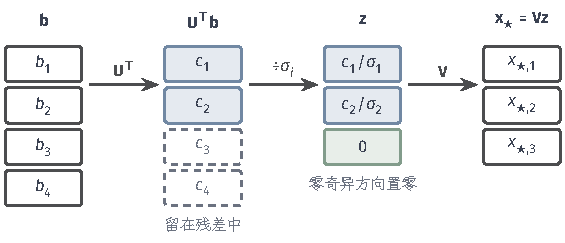
\includegraphics[width=95.652mm]{figures/01-basic-mathematics/03-vectors-matrices-and-multivariate-functions/tikz/c5-svd-solve-coordinates/figure.pdf}
  \caption{SVD求解的坐标变换，示意$m=4$、$d=3$、$r=2$。右端先变到左奇异坐标，蓝色的前$r$个坐标可以拟合，虚线框中的其余坐标无论怎样选$\bm x$都留在残差中；可拟合坐标除以对应奇异值，零奇异方向的坐标取零；最后由右奇异向量还原为原变量。}
  \label{fig:ls-svd-solve-coordinates}
\end{figure}

\paragraph{目标在奇异坐标下分离}
把未知量和右端分别换到右、左奇异坐标，令
\begin{equation}
 \bm z=\bm V^\top\bm x,\qquad \bm c=\bm U^\top\bm b .
 \label{eq:ls-svd-coordinates}
\end{equation}
由$\bm A\bm x=\bm U\bm\Sigma\bm z$，残差变为
\[
 \bm b-\bm A\bm x=\bm U(\bm c-\bm\Sigma\bm z),
\]
其中
\[
 \bm c-\bm\Sigma\bm z=(c_1-\sigma_1z_1,\ \ldots,\ c_r-\sigma_rz_r,\ c_{r+1},\ \ldots,\ c_m)^\top .
\]
由$\bm U$保持长度，
\begin{equation}
 \begin{aligned}
 \lVert\bm b-\bm A\bm x\rVert_2^2&=\lVert\bm c-\bm\Sigma\bm z\rVert_2^2\\
 &=\sum_{i=1}^r(c_i-\sigma_iz_i)^2+\sum_{i=r+1}^mc_i^2 .
 \end{aligned}
 \label{eq:ls-svd-coordinate-split}
\end{equation}
输入坐标$z_{r+1},\ldots,z_d$根本不出现在目标中。

\paragraph{逐个坐标求解}
式~\eqref{eq:ls-svd-coordinate-split}的各平方项互不耦合，可以分别取最小。对每个正奇异值令$c_i-\sigma_iz_i=0$，得
\begin{equation}
 z_i=\frac{c_i}{\sigma_i},\qquad i=1,\ldots,r ;
 \label{eq:ls-svd-coordinate-solution}
\end{equation}
输出端$i>r$的分量$c_i$无论怎样选$\bm x$都留在残差中。所以最小二乘解的全部自由度恰好是输入零空间方向上的坐标$z_{r+1},\ldots,z_d$。

\paragraph{取最小范数}
再由
\[
 \lVert\bm x\rVert_2=\lVert\bm V\bm z\rVert_2=\lVert\bm z\rVert_2 ,
\]
令全部自由坐标为零就使范数最小，得到
\begin{equation}
 \bm x_\star=\sum_{i=1}^r\frac{\bm u_i^\top\bm b}{\sigma_i}\bm v_i .
 \label{eq:ls-svd-solution}
\end{equation}
这给出了执行顺序：先把右端投影到输出奇异方向，再对正奇异值取逆，最后由输入奇异方向重建。它恰是伪逆作用于右端的结果，证明见本节的算法分析。

\subsection{算法实现}

输入是$\bm A\in\mathbb R^{m\times d}$与$\bm b\in\mathbb R^m$，不要求满秩，输出是最小范数最小二乘解$\bm x_\star$，没有额外需要选定的规则。这里按精确的秩$r$描述求解；有限精度下怎样判定数值秩，以及是否截断小奇异值，属于第~\ref{chap:solution-error-regularization}章的内容（第~\ref{sec:ls-pseudoinverse-rank-change}节与第~\ref{sec:ls-tsvd-solve}节）。

算法由两个模块组成：计算SVD取得因子，由奇异坐标求解。

下面用以下数据逐步演示：
\[
 \bm A=\begin{bmatrix}1&1\\1&1\end{bmatrix},\qquad
 \bm b=\begin{bmatrix}1\\3\end{bmatrix}.
\]
两个方程要求$x_1+x_2$同时等于$1$和$3$，方程不相容；$\bm A$的秩为$1$，最小二乘解也不唯一。

\subsubsection{计算SVD}
输入$\bm A$，输出$\bm U_r=[\bm u_1,\ldots,\bm u_r]$、$\bm\Sigma_r=\operatorname{diag}(\sigma_1,\ldots,\sigma_r)$与$\bm V_r=[\bm v_1,\ldots,\bm v_r]$。调用数值SVD过程，按第~\ref{chap:singular-value-decomposition}章的形式取得$\bm A=\bm U_r\bm\Sigma_r\bm V_r^\top$，其中$r=\operatorname{rank}\bm A$，$\bm U_r$与$\bm V_r$的列标准正交，各$\sigma_i>0$。若$\bm A=\bm0$，则直接取$\bm x_\star=\bm0$并结束。

例中$\bm A$的秩为$r=1$，唯一的正奇异值为$\sigma_1=2$，
\[
 \bm A=2\,\bm u_1\bm v_1^\top,\qquad
 \bm u_1=\bm v_1=\frac1{\sqrt2}\begin{bmatrix}1\\1\end{bmatrix};
\]
补齐后的另一对奇异方向
\[
 \bm u_2=\bm v_2=\frac1{\sqrt2}\begin{bmatrix}1\\-1\end{bmatrix}
\]
对应零奇异值，不进入薄分解。

\subsubsection{由奇异坐标求解}
输入$\bm U_r$、$\bm\Sigma_r$、$\bm V_r$与$\bm b$，输出$\bm x_\star$。
\begin{enumerate}
 \item \textbf{投影右端。}对$i=1,\ldots,r$计算
 \[
  c_i=\bm u_i^\top\bm b ,
 \]
 把右端投影到能够拟合的输出方向上；$\bm b$在其余方向上的部分，无论怎样选$\bm x$都会留在残差中。

 例中可拟合分量与被舍弃方向上的分量分别为
 \[
  c_1=\bm u_1^\top\bm b=2\sqrt2,\qquad \bm u_2^\top\bm b=-\sqrt2 .
 \]

 \item \textbf{按奇异值缩放。}根据主要思想中的逐个坐标求解，对$i=1,\ldots,r$计算
 \[
  z_i=\frac{c_i}{\sigma_i} .
 \]
 除法只对正奇异值进行，零奇异值对应的坐标取零。

 例中
 \[
  z_1=\frac{2\sqrt2}2=\sqrt2 .
 \]

 \item \textbf{还原原变量。}根据式~\eqref{eq:ls-svd-solution}，计算
 \[
  \bm x_\star=\bm V_r\bm z=\sum_{i\leq r}z_i\bm v_i .
 \]
 
 例中
 \[
  \bm x_\star=\sqrt2\cdot\frac1{\sqrt2}\begin{bmatrix}1\\1\end{bmatrix}=\begin{bmatrix}1\\1\end{bmatrix}.
 \]

 \item \textbf{输出并核验。}输出$\bm x_\star$，并用原始数据检查$\bm A^\top(\bm b-\bm A\bm x_\star)=\bm0$与$\bm x_\star\perp\ker\bm A$。

 例中拟合值与残差为
 \[
  \bm A\bm x_\star=\begin{bmatrix}2\\2\end{bmatrix},\qquad
  \bm b-\bm A\bm x_\star=\begin{bmatrix}-1\\1\end{bmatrix}.
 \]
 拟合值取两个观测的平均，残差与列空间方向$(1,1)^\top$正交，长度$\sqrt2$等于被舍弃分量的绝对值$\lvert\bm u_2^\top\bm b\rvert$。

 另一方面，$\bm x_\star$与核方向$(1,-1)^\top$正交：全部最小二乘解为$(1+t,1-t)^\top$，范数平方为
 \[
  (1+t)^2+(1-t)^2=2+2t^2 ,
 \]
 $t=0$时最小。
\end{enumerate}
整个过程只用到因子对向量的作用，无需形成完整的伪逆。

\subsection{算法分析}

\paragraph{正确性}
上述过程算出的正是伪逆作用于右端的结果。

\begin{theorem}[SVD求解给出\texorpdfstring{$\bm A^\dagger\bm b$}{A+b}]
\label{thm:ls-svd-solve}
对任意$\bm A\in\mathbb R^{m\times d}$与$\bm b\in\mathbb R^m$，上述过程的输出$\bm x_\star=\bm A^\dagger\bm b$，它是唯一的最小范数最小二乘解。
\end{theorem}
\begin{proof}
由式~\eqref{eq:matrix-analysis-pseudoinverse}，
\[
 \bm A^\dagger\bm b=\sum_{i\leq r}\frac{\bm v_i\bm u_i^\top\bm b}{\sigma_i},
\]
与输出相同；$\bm A=\bm0$时两者都是$\bm0$。最优性由定理~\ref{thm:matrix-analysis-pseudoinverse-minimum-norm}给出。也可以直接验证：残差$\bm b-\bm A\bm x_\star=\bm b-\bm U_r\bm U_r^\top\bm b$与列空间正交，所以$\bm x_\star$满足正规方程；$\bm x_\star\in\operatorname{range}(\bm V_r)=(\ker\bm A)^\perp$，由定理~\ref{thm:ls-minimum-norm-representative}，它在全部最小二乘解中范数最小。
\end{proof}

\paragraph{数值敏感度}
敏感性来自除以小奇异值。固定$\bm A$且$r>0$时，右端扰动$\delta\bm b$使解改变
\begin{equation}
 \begin{gathered}
 \delta\bm x_\star=\sum_{i=1}^r\frac{\bm u_i^\top\delta\bm b}{\sigma_i}\bm v_i,\\
 \lVert\delta\bm x_\star\rVert_2\leq\frac{\lVert\delta\bm b\rVert_2}{\sigma_r},
 \end{gathered}
 \label{eq:ls-svd-perturbation-bound}
\end{equation}
即放大倍数至多为$1/\sigma_r$。

稳定地算出SVD并不能消除问题本身的病态：分解残差很小，恢复出的系数仍可能被观测误差严重放大。若为了压低放大而截去真实的正奇异值，求的就已不是$\bm A^\dagger\bm b$，这属于第~\ref{chap:solution-error-regularization}章的截断SVD与正则化。

\subsection{加权最小二乘}
\label{sec:ls-weighted-svd-solve}

\subsubsection{主要思想}
第~\ref{sec:ls-weighted-ls}节的加权最小二乘以对称正定的权矩阵$\bm M\in\mathbb R^{m\times m}$规定目标函数$(\bm A\bm x-\bm b)^\top\bm M(\bm A\bm x-\bm b)$。核心思想是把权矩阵写成$\bm M=\bm R^\top\bm R$，代入目标函数得
\begin{equation}
 \begin{aligned}
 (\bm A\bm x-\bm b)^\top\bm M(\bm A\bm x-\bm b)
 &=\bigl(\bm R(\bm A\bm x-\bm b)\bigr)^\top\bigl(\bm R(\bm A\bm x-\bm b)\bigr)\\
 &=\lVert\bm R\bm A\bm x-\bm R\bm b\rVert_2^2 .
 \end{aligned}
 \label{eq:ls-weighted-whitening}
\end{equation}
所以用同一个$\bm R$变换$\bm A$和$\bm b$，记
\begin{equation}
 \widetilde{\bm A}=\bm R\bm A,\qquad \widetilde{\bm b}=\bm R\bm b ,
 \label{eq:ls-weighted-transformed-data}
\end{equation}
问题就成为普通最小二乘，对它调用SVD求解得到$\widetilde{\bm A}^\dagger\widetilde{\bm b}$。这一步称为白化。

$\bm R$的取法由$\bm M=\bm R^\top\bm R$决定。若Cholesky分解写作$\bm M=\bm L\bm L^\top$，必须取
\begin{equation}
 \bm R=\bm L^\top ,
 \label{eq:ls-weighted-cholesky-factor}
\end{equation}
才有$\bm R^\top\bm R=\bm L\bm L^\top$；取$\bm R=\bm L$则得到$\bm L^\top\bm L$，一般不等于$\bm M$。

对角权$\bm M=\operatorname{diag}(w_1,\ldots,w_m)$直接取
\begin{equation}
 \bm R=\operatorname{diag}(\sqrt{w_1},\ldots,\sqrt{w_m}) .
 \label{eq:ls-weighted-diagonal-factor}
\end{equation}

若权以$\bm M=\bm\Gamma^{-1}$的形式给出，$\bm\Gamma$为对称正定矩阵（例如观测误差的协方差），就分解$\bm\Gamma=\bm L\bm L^\top$，这时
\begin{equation}
 \bm M=\bm L^{-\top}\bm L^{-1},\qquad \bm R=\bm L^{-1},
 \label{eq:ls-weighted-covariance-factor}
\end{equation}
$\widetilde{\bm A}$与$\widetilde{\bm b}$由
\begin{equation}
 \bm L\widetilde{\bm A}=\bm A,\qquad \bm L\widetilde{\bm b}=\bm b
 \label{eq:ls-weighted-covariance-solve}
\end{equation}
按式~\eqref{eq:ls-forward-substitution}前代求出，不显式求逆。

变换只作用于观测端，未知量$\bm x$本身没有改变，所以白化后的解无须再变换回去；它为什么正是加权最小二乘解中欧氏范数最小的代表，见本小节的算法分析。权矩阵度量的是残差，不是系数，所以不能再把它当成系数范数的权重。

\subsubsection{算法实现}
输入是$\bm A$、$\bm b$与权矩阵$\bm M$，输出是加权最小二乘解中欧氏范数最小的代表$\bm x_\star$，没有额外需要选定的规则。

下面用以下数据逐步演示：
\[
 \bm A=\begin{bmatrix}1&1\\1&1\end{bmatrix},\qquad
 \bm b=\begin{bmatrix}0\\2\end{bmatrix},
\]
权矩阵为
\[
 \bm M=\begin{bmatrix}1&0\\0&3\end{bmatrix}.
\]
系数矩阵与第~\ref{sec:ls-svd-solve}节算法实现的例子相同，秩为$1$，加权解不唯一，两个观测的权重之比为$1:3$。
\begin{enumerate}
 \item \textbf{构造权因子。}按主要思想中的三种形式之一取得$\bm R$：一般情形作Cholesky分解$\bm M=\bm L\bm L^\top$并取$\bm R=\bm L^\top$，对角权取各权重的平方根，协方差形式分解$\bm\Gamma$。

 例中权为对角的，
 \[
  \bm R=\operatorname{diag}(1,\sqrt3) .
 \]

 \item \textbf{白化数据。}根据式~\eqref{eq:ls-weighted-whitening}，计算$\widetilde{\bm A}=\bm R\bm A$与$\widetilde{\bm b}=\bm R\bm b$；协方差形式改用前代。

 例中
 \[
  \widetilde{\bm A}=\begin{bmatrix}1&1\\\sqrt3&\sqrt3\end{bmatrix},\qquad
  \widetilde{\bm b}=\begin{bmatrix}0\\2\sqrt3\end{bmatrix}.
 \]

 \item \textbf{求解白化后的问题。}对$(\widetilde{\bm A},\widetilde{\bm b})$调用第~\ref{sec:ls-svd-solve}节的SVD求解，得到$\bm x_\star$并输出；$\widetilde{\bm A}$满列秩时也可以调用第~\ref{sec:ls-qr-method}节的QR求解。
 
 例中
 \[
  \widetilde{\bm A}=\begin{bmatrix}1\\\sqrt3\end{bmatrix}\begin{bmatrix}1&1\end{bmatrix},
 \]
 秩为$1$，唯一的正奇异值为
 \[
  \tilde\sigma_1=\lVert(1,\sqrt3)\rVert_2\,\lVert(1,1)\rVert_2=2\sqrt2,
 \]
 左、右奇异向量为
 \[
  \tilde{\bm u}_1=\frac12\begin{bmatrix}1\\\sqrt3\end{bmatrix},\qquad
  \tilde{\bm v}_1=\frac1{\sqrt2}\begin{bmatrix}1\\1\end{bmatrix}.
 \]
 投影与缩放得
 \[
  \tilde{\bm u}_1^\top\widetilde{\bm b}=3,\qquad
  z_1=\frac{3}{2\sqrt2},
 \]
 还原得
 \[
  \bm x_\star=\frac{3}{2\sqrt2}\cdot\frac1{\sqrt2}\begin{bmatrix}1\\1\end{bmatrix}=\begin{bmatrix}3/4\\3/4\end{bmatrix}.
 \]

 \item \textbf{核验。}用原始数据检查加权正规残差$\bm A^\top\bm M(\bm b-\bm A\bm x_\star)=\bm0$，需要最小范数时再检查$\bm x_\star\perp\ker\bm A$。

 例中拟合值为
 \[
  \bm A\bm x_\star=\begin{bmatrix}3/2\\3/2\end{bmatrix},
 \]
 两个观测的拟合值相同，取的是$0$与$2$按权重$1:3$的加权平均，而不是普通平均$1$。原残差及其加权为
 \[
  \bm r=\begin{bmatrix}-3/2\\1/2\end{bmatrix},\qquad
  \bm M\bm r=\begin{bmatrix}-3/2\\3/2\end{bmatrix},
 \]
 所以
 \[
  \bm A^\top\bm M\bm r=\bm0,\qquad
  \bm r^\top\bm M\bm r=\tfrac94+3\cdot\tfrac14=3 ,
 \]
 后者是加权残差平方。系数差的方向$(1,-1)^\top$张成$\ker\bm A$，$\bm x_\star$在这个方向上的分量为零。
\end{enumerate}

\subsubsection{算法分析}
由式~\eqref{eq:ls-weighted-whitening}，变换前后的目标函数逐点相等；未知量及其欧氏范数也没有变，所以两个问题的最优解集与最小范数代表都相同（定理~\ref{thm:ls-weighted-least-squares}）。又$\bm R$可逆，$\ker\widetilde{\bm A}=\ker\bm A$，所以$\bm x_\star\perp\ker\bm A$。

数值敏感度取决于$\widetilde{\bm A}=\bm R\bm A$而不是$\bm A$：权重可能改善条件，也可能使它变差，应在变换后的系统上判断。

\subsection{齐次最小二乘}
\label{sec:ls-homogeneous-svd-solve}

\subsubsection{主要思想}
第~\ref{sec:linear-algebra-homogeneous-estimation}节的齐次最小二乘在$\lVert\bm x\rVert_2=1$的约束下最小化$\lVert\bm A\bm x\rVert_2$。它是$\bm b=\bm0$的情形，单位长度约束属于求解目标，用来排除无意义的零解。核心思想是选择被$\bm A$伸缩得最小的方向。

用完整的右奇异基$\bm V=[\bm v_1,\ldots,\bm v_d]$写$\bm x=\bm V\bm z$。记$\hat\sigma_i=\lVert\bm A\bm v_i\rVert_2$为第$i$个方向的伸缩量：$i\leq\min(m,d)$时它是第$i$个奇异值（可以为零），$m<d$时多出的$d-m$个方向属于零空间，伸缩量为零。

由SVD，$\bm A\bm v_i=\hat\sigma_i\bm u_i$（伸缩量为零时为$\bm0$），各$\bm A\bm v_i$两两正交，于是约束与目标分别化为
\begin{equation}
 \lVert\bm x\rVert_2^2=\sum_{i=1}^dz_i^2=1,\qquad
 \lVert\bm A\bm x\rVert_2^2=\sum_{i=1}^d\hat\sigma_i^2z_i^2 .
 \label{eq:ls-homogeneous-coordinates}
\end{equation}
第二式是平方伸缩量$\hat\sigma_i^2$以$z_i^2$为权的加权平均，权的和为$1$，所以它不小于其中最小的一个$\hat\sigma_d^2$；把全部权放在最后一个坐标上就达到这个最小值，即
\begin{equation}
 \bm z=\pm\bm e_d,\qquad \hat{\bm x}=\bm V\bm z=\pm\bm v_d .
 \label{eq:ls-homogeneous-solution}
\end{equation}
最小值何时还在别的方向上达到，见本小节的算法分析。

\subsubsection{算法实现}
输入是$\bm A\in\mathbb R^{m\times d}$，输出是使$\lVert\bm A\bm x\rVert_2$最小的单位向量$\hat{\bm x}$，没有额外需要选定的规则。

下面用以下矩阵逐步演示：
\[
 \bm A=\begin{bmatrix}3&0\\0&1\\0&0\end{bmatrix}.
\]

\begin{enumerate}
 \item \textbf{计算完整右奇异基。}调用数值SVD过程，取得第~\ref{chap:singular-value-decomposition}章中的完整右因子$\bm V$，各列按伸缩量从大到小排列，并检查输入维数与秩。
 
 $m<d$时奇异值只有$m$个，完整右基中多出的方向属于零空间，也要保留；薄SVD可能没有列出全部右零空间，必须补齐相应的基，不能机械地取薄SVD的最后一列。
 
 这些方向直接从$\bm A$的SVD取得，不通过显式形成$\bm A^\top\bm A$再求特征向量。
 
 例中$\bm A$的两列已经正交，
 \[
  \sigma_1=3,\qquad \sigma_2=1,\qquad \bm V=\bm I,\quad\text{即}\quad \bm v_1=\bm e_1,\ \bm v_2=\bm e_2 ;
 \]
 $m>d$，无须补齐。

 \item \textbf{取最后一列。}令$\hat{\bm x}=\bm v_d$并输出：存在零空间时它是零空间中的单位向量，否则是最小正奇异值的右奇异向量。它已经是单位向量，无须再归一化；$\hat{\bm x}$与$-\hat{\bm x}$表示同一组参数比例。

 例中
 \[
  \hat{\bm x}=\bm e_2=\begin{bmatrix}0\\1\end{bmatrix},\qquad
  \lVert\bm A\hat{\bm x}\rVert_2=1 .
 \]

 \item \textbf{核验。}检查$\lVert\hat{\bm x}\rVert_2=1$，以及$\lVert\bm A\hat{\bm x}\rVert_2$等于最小伸缩量。

 例中在约束$x_1^2+x_2^2=1$下，目标为
 \[
  \lVert\bm A\bm x\rVert_2^2=9x_1^2+x_2^2=1+8x_1^2 ,
 \]
 在$x_1=0$时最小，最小残差范数为$1$，与$\hat{\bm x}=(0,\pm1)^\top$一致。零向量虽然给出零残差，却不满足单位长度约束。
\end{enumerate}

\subsubsection{算法分析}
正确性直接来自定理~\ref{thm:ls-homogeneous-minimizers}：$\lVert\bm A\bm x\rVert_2^2=\bm x^\top\bm A^\top\bm A\bm x$在单位球面上的最小值是$\bm A^\top\bm A$的最小特征值，由对应的特征向量达到，而$\bm v_d$正是这样的向量。

式~\eqref{eq:ls-homogeneous-coordinates}的加权平均论证给出同一结论，并刻画了全部最优解：加权平均等于最小值，当且仅当$\bm z$只落在取得最小伸缩量的那些坐标上。

所以最小伸缩量是单重的时，实数域中的最优方向只有$\pm\bm v_d$两个；重数大于一或零空间多于一维时，最优解是相应子空间中的全部单位向量，$\bm v_d$只是其中一个选择，应报告整个最优子空间，而不是声称有唯一的向量。

最优方向的敏感度由最小特征值与其余谱之间的间隙控制，可用第~\ref{sec:ls-subspace-sensitivity}节的子空间扰动界估计。单位长度与最优性的检验按第~\ref{sec:ls-least-squares-verification}节进行。
